% Minimal TikZ standalone example
\documentclass[tikz, border=1mm]{standalone}

\usepackage{amsmath}

\usetikzlibrary{calc}
\usetikzlibrary{angles,quotes}

\begin{document}
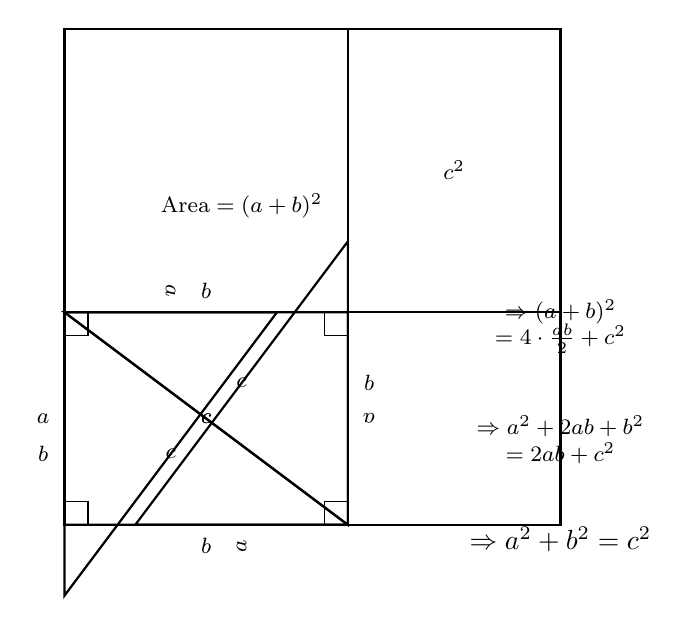
\begin{tikzpicture}[scale=0.9, font=\footnotesize]

% Right triangle dimensions (legs a=3, b=4, hyp c=5 example)
\def\a{3}
\def\b{4}
\def\c{5}

% Outer square: side = a+b
\draw[thick] (0,0) rectangle (\a+\b, \a+\b);
\node at (2.5,4.5) {$\text{Area} = (a+b)^2$};

% Four right triangles
\foreach \x/\y/\ang  in {0/0/0, \b/0/90, \b/\a/180, 0/\a/270} {
	\begin{scope}[shift={(\x,\y)}, rotate=\ang]
		\draw[thick] (0,0) -- (\b,0) -- (0,\a) -- cycle;
		\node at (\b/2,-0.3) {$b$};
		\node[rotate=\ang] at (-0.3,\a/2) {$a$};
		\node at (\b/2,\a/2) {$c$};
		\coordinate (O) at (0,0);
		\coordinate (X) at (\b,0);
		\coordinate (Y) at (0,\a);
		\draw pic["", draw, angle radius=3mm] {right angle=Y--O--X};
	\end{scope}
	}

% Inner square
\draw[thick] (\b,\a) ++(0,0)
  -- +( \a,0) -- +( \a,\b)
  -- +(0,\b) -- cycle;
\node at (\b+\a/2,\a+\b/2) {$c^2$};

% Equations (extra explanation)
\node[align=center] at (7,2.8) {$\Rightarrow (a+b)^2$ \\ $ = 4\cdot\frac{ab}{2} + c^2$};
\node[align=center] at (7,1.2) {$\Rightarrow a^2 + 2ab + b^2$ \\ $ = 2ab + c^2$};
\node[align=center, font=\bfseries] at (7,-0.2)
  {$\Rightarrow a^2 + b^2 = c^2$};

\end{tikzpicture}
\end{document}
